\documentclass[10pt,pdftex,twoside,onecolumn,a4paper,openright]{book}

\usepackage{istthesis}

\newcommand{\degree}{\ensuremath{^\circ}} % degree symbol

\title{My dear project}
\author{Manel Esteves dos Santos Pereira}
\submitdate{Julho 1900}
\copyrightyear{1900}
\thesisadvisor{Nome do coordenador}{1}
%\thesisadvisor{Ricardo Lopes Pereira}{1}
%\thesisadvisor{Teresa Vazão}{1}
%\thesisadvisor{António Varela}{1}
\currentdegree{Licenciado em Engenharia Informática e de Computadores}
\thesisdepartment{Departamento de Engenharia Informática}
\thesiscourse{Engenharia Informática e de Computadores}
\thesisdegree{Mestre}
\thjuri[Prof. Doutor Nome do Presidente do Júri][Prof. Doutor Nome do Vogal 1]

\begin{document}

\selectlanguage{english}

\beforepreface
\chapter*{Abstract}

% DO NOT CHANGE THIS - Add entry in the table of contents as chapter
\addcontentsline{toc}{chapter}{Abstract}

% TODO
The abstract describes the objective, the content of the work and its counclusion. Use a maximum of around 250 words.

\vspace{1cm}

% TODO 4 to 6 keywords;
\textbf{\Large Keywords:} keyword1, keyword2,...

\cleardoublepage


\cleardoublepage
\chapter*{Resumo}

% DO NOT CHANGE THIS - Add entry in the table of contents as chapter
\addcontentsline{toc}{chapter}{Resumo}

% TODO
O resumo analítico descreve o objectivo, o conteúdo do trabalho e as conclusões, também designado por resumo ou abstract, deve ser escrito em português e inglês, com um máximo de 250 palavras cada.

\vspace{1cm}

% TODO - 4 a 6 palavras-chave;
\textbf{\Large Palavras-chave:} palavra-chave1, palavra-chave2,...

\cleardoublepage


\cleardoublepage
\chapter*{\acknowledgments}

% Add entry in the table of contents as chapter
\addcontentsline{toc}{chapter}{\acknowledgments}

A few words about the university, financial support, research advisor, dissertation readers, faculty or other professors, lab mates, other friends and family...

\cleardoublepage


\cleardoublepage

\afterpreface

\chapter{Introduction}\label{introduction}

\section{Background}
Nesta secção devem descrever a área em que a vossa tese se insere, de forma
a contextualizar o problema que vão resolver. No âmbito da área devem
identificar os principais problemas que existem.


\section{Proposed Solution}
Nesta secção devem identificar objectivamente o problema que vão resolver e o
tipo de solução que vão adoptar.

Exemplos de problemas que podem ser endereçados e tipos de soluções:

\begin{itemize}
\item Esta situação ainda não tem solução - > vou propor uma nova
\item Existem soluções para aspectos específicos, mas não existe uma que integre
os vários aspectos -> vou integrar as várias
\item Existem demonstrações matemáticas ou validações por simulação, mas
será que funcionam na realidade (quando as aproximações que se fizerem
deixarem de ser válidas) - > vou fazer um protótipo experimental
\item Existem demasiadas propostas de soluções, validadas em diferentes
condições –> vou fazer um estudo comparativo que as avalie sob diferentes
perspectivas
\item Existe uma boa solução, mas com um desempenho variável em função da
configuração- > vou fazer um estudo que permita verificar em que medida é
possível ajustar os parâmetros automaticamente às diferentes situações.
\item Existe uma teccnologia que ainda não está devidamente explorada -> vou
fazer um protótipo de ilustre o seu uso.
\end{itemize}

\section{Thesis Contribution}
Nesta secção devem identificar como é que a vossa solução vai contribuir para
resolver o problema.

\section{Outline}

This document describes the research and work developed and it is organized as follows:

\begin{itemize}
\item \textbf{Chapter \ref{introduction}} presents the motivation, background and proposed solution.
\item \textbf{Chapter \ref{relatedwork}} describes the previous work in the field.
\item \textbf{Chapter \ref{architecture}} describes the system requirements and the architecture of GBus.
\item \textbf{Chapter \ref{implementation}} describes the implementation of GBus and the technologies chosen.
\item \textbf{Chapter \ref{evaluation}} describes the evaluation tests performed and the corresponding results.
\item \textbf{Chapter \ref{conclusion}} summarizes the work developed and future work.
\end{itemize}


\cleardoublepage

\chapter{Related Work}
\label{chapter:relatedwork}

Nesta secção devem apresentar o que andaram a ler. A estrutura depende muito do
vosso trabalho/abordagem, mas deve sempre começar por uma apresentação da
estruturação seguida. Posteriormente, devem apresentar cada item numa secção
diferente. Exemplos de estruturações:
\begin{itemize}
\item normas, trabalhos científicos e ferramentas comerciais;
\item trabalhos da área B, da área C, etc...
\end{itemize}
Podem terminar cada secção com uma pequena avaliação comparativa.
No final do capítulo devem fazer uma síntese. Esta síntese pode vir acompanhada
duma tabela com as várias soluções, as várias características que vos interessam
e com a indicação das soluções que satisfazem as vossas necessidades. Podem
terminar a secção sumariando o vosso trabalho numa frase.

Exemplo de referencia~\cite{Biagioni2011}.


\cleardoublepage

\chapter{Architecture}
\label{chapter:architecture}
Esta secção deve englobar:

\begin{itemize}
    \item Uma análise de requisitos, onde devem “abrir” portas para as principais
        características da vossa arquitectura.
    \item Uma descrição de alto nível da arquitectura do vosso sistema. Esta descrição
        pode ser:
        \begin{itemize}
            \item A arquitectura de rede, explicando os principais componentes e as
                funções que executam.
            \item A arquitectura de SW da aplicação, explicando os principais
                componentes e as funções que executam.
        \end{itemize}
    \item Descrições detalhadas de todos os componentes da vossa arquitectura.
    \item As escolhas que efectuarem em termos de arquitectura global e de detalhe,
        devem ser justificadas, face aos requisitos que identificaram.
\end{itemize}

Sempre que possível, ilustrem a arquitectura com figuras, que descrevam
sucintamente o modelo como na Figure~\ref{fig:logoCNM}.

\begin{figure}[!htb]
  \centering
  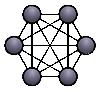
\includegraphics[width=0.25\textwidth]{Figures/logoCNM.png}
  \caption[Caption for figure in TOC]{Caption for figure.}
  \label{fig:logoCNM}
\end{figure}

\cleardoublepage

\chapter{Implementation}
\label{chapter:implementation}

\section{Implementation Options}
Neste secção devem apresentar as opções de implementação que tinham ao vosso
dispor, avaliá-las e justificar a escolha que realizaram. Isto pode englobar:
\begin{itemize}
    \item Simuladores
    \item Linguagens e ambientes de programação
    \item Sistemas operativos
    \item Hardware
\end{itemize}
Fica sempre bem na avaliação colocar uma tabela com as características
pretendidas e as que são satisfeitas pelas várias opções (tipo catálogo com as
características dos automóveis). A escolha deve surgir naturalmente, com base na
opção que tem mais cruzes\ldots

\section{Architecture}
Nesta secção devem explicar como implementaram a vossa solução, apresentando
as simplificações que efectuaram, face ao modelo inicialmente previsto. As
simplificações devem ser devidamente justificadas. Se for possível, devem indicar
que estas não põem em causa as contribuições da tese.
Podem ainda descrever os principais problemas que tiveram e a forma como os
abordaram e resolveram.

Se estiverem a usar um simulador devem:

\begin{itemize}
    \item explicar o funcionamento do simulador
    \item explicar as alterações e modelos que desenvolveram no simulador e que permitem validar a vossa ideia
\end{itemize}

Se estiveram a desenvolver SW, sem simulador devem:
\begin{itemize}
    \item explicar os módulos, interfaces, estruturas de dados, etc\ldots
\end{itemize}

Sempre que possível, ilustrem a arquitectura com figuras que demonstrem a
evolução face à arquitectura da secção anterior. Isto é, usem as figuras anteriores
e façam as modificações necessárias à obtenção da arquitectura do protótipo.
\ldots

\cleardoublepage

\chapter{Evaluation}
\label{chapter:evaluation}

\section{Tests Objectives}
Nesta secção devem descrever os objectivos dos testes que realizaram, explicitando
que a razão pela qual os testes são relevantes face à validação das contribuições da
tese.

\section{Tests Scenarios}
Nesta secção devem descrever o cenário de teste, incluindo, por exemplo, a
definição da rede, o modelo de tráfego, as características de cada elemento....
A descrição deve ser feita, de forma a que os testes possam ser reprodutíveis.
Se os testes forem feitos em ambiente real devem ser descritas as características
dos equipamentos, memória, CPU, disco, SO, etc....

Devem também descrever as características das experiências, do ponto de vista
estatístico. Número de testes realizados, grandezas que vão ser medidas, formas de
medição dos valores, etc...

Sempre que possível, ilustrem o cenário de testes com figuras e com tabelas, que
descrevam sucintamente o modelo.

\section{Test Results}
Nesta secção devem apresentar os resultados dos testes, quer sobre a forma
de tabelas, quer sobre a forma de gráficos. As tabelas e os gráficos devem ser
apresentados e depois analisados, detalhadamente.
\ldots

Here is an example of a table~\ref{table:simple}.

\begin{table}[!htb]
  \begin{center}
  \caption[Table caption shown in TOC]{Table caption}
    \begin{tabular}{|c|c|}
      \hline
      item 1 & item 2 \\
      \hline
      item 3 & item 4 \\
      \hline
    \end{tabular}
  \end{center}
  \label{table:simple}
\end{table}

\cleardoublepage

\chapter{Conclusion}\label{conclusion}

\section{Summary}
Neste secção deve-se fazer o resumo do trabalho efectuado, retomando a ideia, as
contribuições definidas e a forma como estas se materializaram

\section{Conclusions}
Nesta secção devem ser retiradas conclusões do trabalho realizado, em face dos
resultados obtidos.

\section{Future Work}
Nesta secção devem identificado o trabalho futuro, sob duas perspectivas:

\begin{itemize}
\item o trabalho que resulta directamente dos problemas que a vossa proposta criou, ou não conseguiu resolver
\item o trabalho que resulta da evolução do sistemas
\end{itemize}

\cleardoublepage


%\bibliographystyle{jmb}   % For references with authors name Joao et al (1984)
\bibliographystyle{splncs} % For references with number [1]

\addcontentsline{toc}{chapter}{Bibliography}
\bibliography{bibliography}

\addcontentsline{toc}{chapter}{Appendix}
\appendix
\chapter{Vector calculus}
\label{chapter:appendix}

Use to include images/diagrams tables which are important but were to big to include in the main tex.

Note that in no case the document can exceed a total of 100 pages.

Some equations examples:

\section{Vector identities}
\label{section:vectorIdentities}

\begin{equation}
	\nabla \times \left( \nabla \phi \right) = 0
	\label{eq:cross_nnp}
\end{equation}

\begin{equation}
	\nabla \cdot \left( \nabla \times {\bf u} \right) = 0
	\label{eq:dotCross_nnu}
\end{equation}

\cleardoublepage



\end{document}
